\begin{table*}[t]
\centering
\resizebox{0.94\textwidth}{!}{
\begin{tabular}{lcccccccc}
\toprule
    \textbf{Model} & \textbf{GSM8K} & \textbf{MATH-500} & \textbf{AIME2024} & \textbf{AIME2025} & \textbf{AMC2023} & \textbf{OlympiadBench} & \textbf{AVG} \\
    \midrule
    LLaMA-3.1-8B-Base~\citep{dubey2024llama} & 7.58 & 3.20 & 0.00 & 0.00 & 4.22 & 1.19 & 2.70 \\
    \rowcolor{new_green!15}
    \texttt{\ \ + 20K Qwen-Distill-Data} & 62.47 & 29.40 & 0.00 & 0.00 & 12.81 & 6.81 & 18.58 \\
    \rowcolor{new_blue!15}
    \texttt{\ \ + 20K OSS-Distill-Data} & 75.89 & 54.20 & 4.38 & 6.46 & 37.34 & 23.85 & 33.69 \\
    \rowcolor{new_blue!15}
    \texttt{\ \ + 20K QwQ-Distill-Data} & 64.53 & 32.20 & 2.92 & 0.42 & 16.72 & 8.89 & 20.95 \\
    \rowcolor{new_purple!15}
    \texttt{\ \ + 20K OSS-\method{}} & 67.85  & 35.20  & 1.83  & 0.83  & 20.53  & 11.11  & 22.89 \\
    \rowcolor{new_purple!15}
    \texttt{\ \ + 20K QwQ-\method{}} & 66.41  & 35.00  & 2.08  & 0.63  & 20.16  & 10.37  & 22.44 \\
    \midrule
    Llama-3.1-8B-Instruct~\citep{dubey2024llama} & 75.89 & 35.20 & 4.17 & 1.04 & 23.59 & 12.00 & 25.32 \\
    \rowcolor{new_green!15}
    \texttt{\ \ + 20K Qwen-Distill-Data} & 76.50 & 39.80 & 4.38 & 1.04 & 25.63 & 19.70 & 27.84 \\
    \rowcolor{new_blue!15}
    \texttt{\ \ + 20K OSS-Distill-Data} & 79.00 & 60.80 & 10.83 & 7.71 & 47.03 & 30.22 & 39.27 \\
    \rowcolor{new_blue!15}
    \texttt{\ \ + 20K QwQ-Distill-Data} & 82.41 & 60.80 & 4.38 & 8.33 & 32.97 & 25.48 & 35.73 \\
    \rowcolor{new_purple!15}
    \texttt{\ \ + 20K OSS-\method{}} & 83.24 & 51.80 & 4.79 & 1.04 & 32.50 & 21.04 & 32.40  \\
    \rowcolor{new_purple!15}
    \texttt{\ \ + 20K QwQ-\method{}} & 84.31 & 50.20 & 5.21 & 1.67 & 32.34 & 20.00 & 32.29  \\
\bottomrule
\end{tabular}
}
\caption{Performance comparison across six benchmarks. Here, ``\raisebox{1pt}{\colorbox{new_purple!15}{ \rule[-0.2ex]{0pt}{1.0ex} }}'': distill from instruction LLMs+\method, ``\raisebox{1pt}{\colorbox{new_blue!15}{ \rule[-0.2ex]{0pt}{1.0ex} }}'': distill from reasoning LLMs, ``\raisebox{1pt}{\colorbox{new_green!15}{ \rule[-0.2ex]{0pt}{1.0ex} }}'': distill from instruction LLMs. See Table~\ref{tab:full_method_result} in Appendix for full results.}
\label{tab:synthesis_results}
\end{table*}

\begin{figure*}[t]
    \centering
    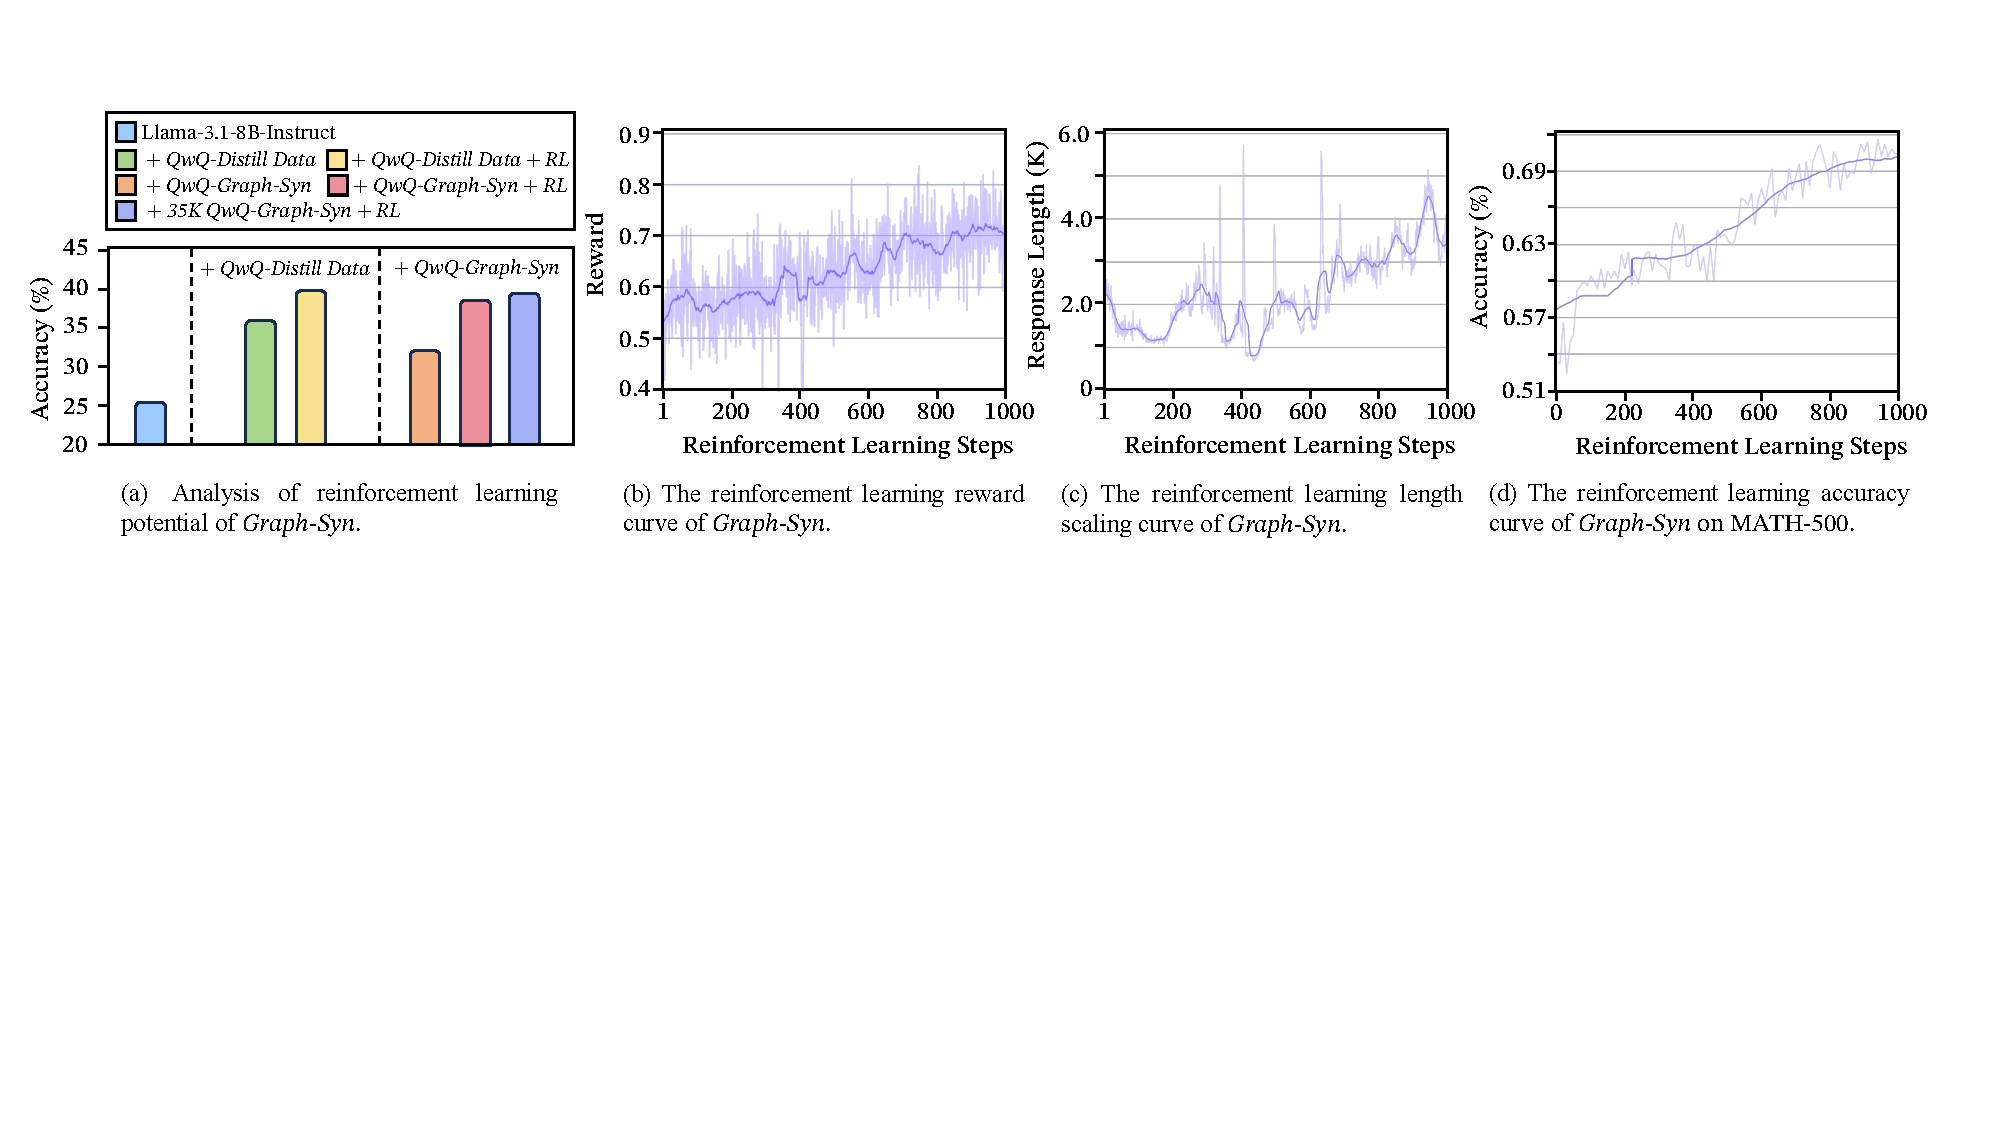
\includegraphics[width=0.98\textwidth]{figures/rl.pdf}
    
    \caption{The continual improvement of RL performance with \method-initialized models. More details about the RL performance are in Table~\ref{tab:rl_results} in Appendix.}
    
    \label{fig:rl}
\end{figure*}

\section{Synthetic Chemistry: Synthesis Long CoT Molecules from Scratch}
LLMs may acquire advanced reasoning partly through exposure to explicit, structured Long CoT reasoning traces. However, it remains unclear how reliably such structures can be induced by prompting an instruction-tuned model, rather than obtained through distillation.\vspace{-8pt}


\paragraph{\textbf{\method Methodology.}}
To address this gap, we propose a synthetic framework, \method, that views targeted reasoning traces as macromolecular structures using only instruction LLMs. This method is a random walk on a transition probability graph in Figure~\ref{fig:transfer} composed of 4 reasoning behaviors from stronger reasoning LLMs that support Long CoT.\vspace{-8pt}


\paragraph{\textbf{\method can synthesize effective bond structures.}}
To test whether Long CoT capabilities can be learned from instruction LLMs, in Table~\ref{tab:synthesis_results}, we conduct training on \method generated data, which even achieves reasoning performance close to QwQ distillation. This suggests that instruction-driven synthesis can induce useful structural regularities, enabling lower-cost behavior transfer.\vspace{-8pt}



\begin{figure*}[t]
    \centering
    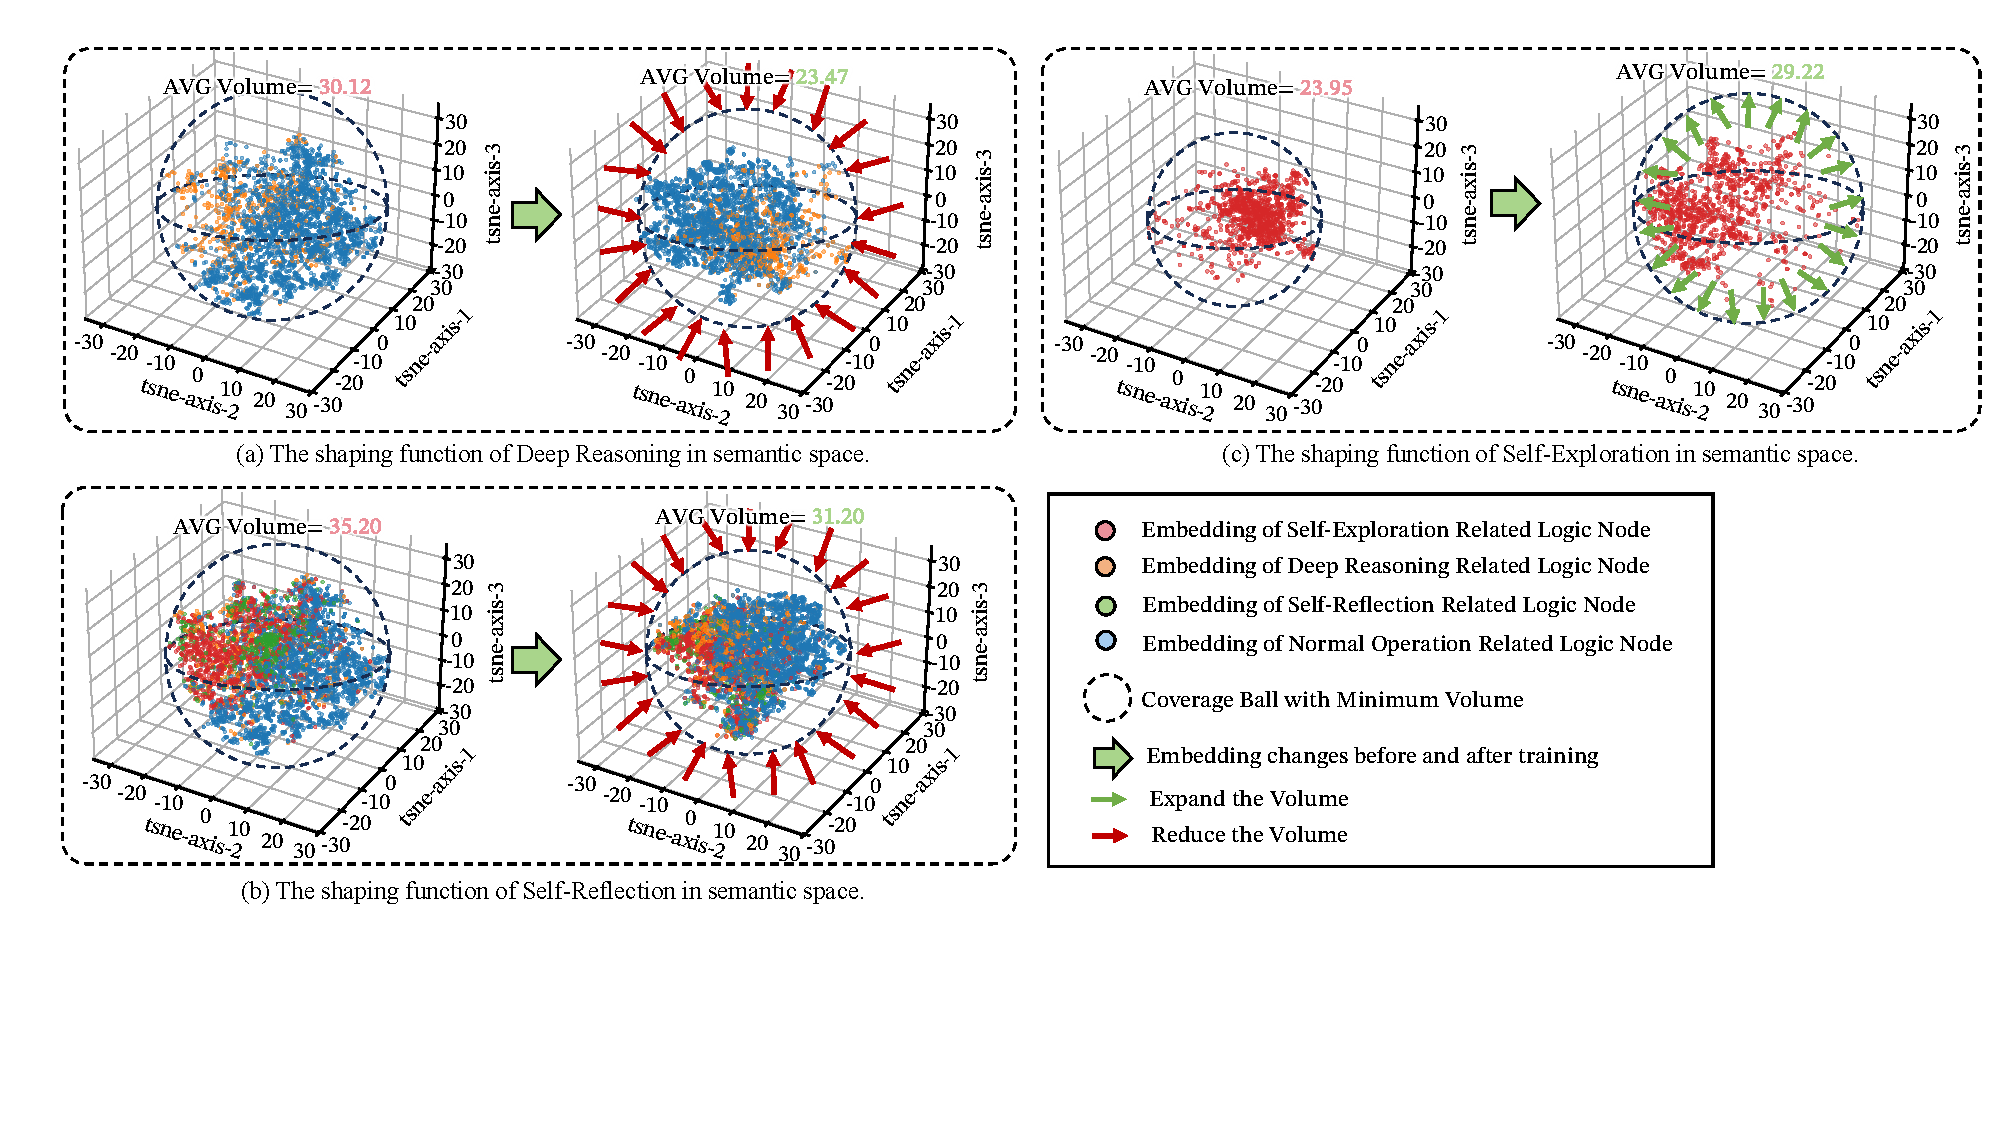
\includegraphics[width=0.98\textwidth]{figures/function.pdf}
    
    \caption{Roles of individual bonds in reasoning, inferred from semantic-space comparisons between Llama-3.1-8B-Instruct and Llama-3.1-8B-Instruct + QwQ-\method. Performance impact is shown in Fig.~\ref{fig:capability} (Appendix).}
    
    \label{fig:function}
\end{figure*}

\paragraph{\textbf{\method can further trigger stronger and continually improving RL.}}
We further evaluate \method-initialized LLMs' potential in reinforcement learning (RL). \method-initialized LLMs outperform those initialized from base LLMs. In Figure~\ref{fig:rl} (a), they show steadier fine-tuning gains, indicating stronger immediate reasoning and more reliable RL adaptation.
Moreover, Figures~\ref{fig:rl} (b-d) show that these gains persist over extended RL training, demonstrating durable benefits from synthesized Long CoT structures.
This effective use under RL supports their practical utility across diverse cognitive tasks.

\begin{TakeawayBox}{Takeaway 4}
\begin{itemize}[leftmargin=16pt, itemsep=0pt, topsep=0pt]
    \item \method{} successfully synthesizes Long CoT structures that match transition distributions from capable teacher models without requiring Long CoT distillation data.
    \item Transition-based Long CoT datasets achieve stable convergence and near-distillation performance, proving effective reasoning structures emerge purely from instruction-level synthesis at lower cost.
    \item Models initialized with synthesized Long CoT weights demonstrate superior and sustained RL performance gains, providing a robust foundation for continual learning in dynamic environments.
\end{itemize} 
\end{TakeawayBox}

